
\subsection{Detection Layer - Bilderkennung}

\subsubsection{Anfertigung der Bilder entlang der Strassen}
Damit das Convnet die Einteilung zwischen Fussgängerstreifen und Nicht-Fussgängerstreifen machen kann, braucht es ein RBG Bild mit 50 x 50 Pixeln als Input. Diese \Gls{Inputbild}er werden aus dem gedownloadetem Orthofoto ausgeschnitten. Mithilfe der Strassenkoordinaten muss nicht das ganze Orthofoto in kleine Bilder aufgeteilt, sondern die Inputbilder können nur entlang der Strassen ausgeschnitten werden. Der Abstand zwischen zwei Inputbildern (auch Schrittweite) ist so gewählt, das eine gewisse Überlappung vorliegt.

\decision{Eckdaten Anfertigung Inputbilder} 
Die Inputbilder für das Convnet sind 50 x 50 Pixel gross, da auf Zoomstufe 19 50 Pixel etwa der Breite von zwei Strassen entspricht. Die Schrittweite wurde so angepasst, dass auch Fussgängerstreifen, die zwischen zwei Inputbildern liegen, erkannt werden.

\begin{figure}[H]
	\centering
	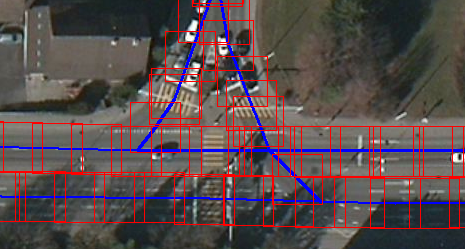
\includegraphics{images/squared_images.png}
	\caption[Anfertigung Inputbilder]{Blau: Strassenverlauf, Rot: Ausgeschnittene Bilder 50 x 50 Pixel. Diese Visualisierung der Inputbilder kann für jede beliebige BBox selbst durchgeführt werden. Siehe dazu examples/VisualizeSquaredImages.py im Projektordner.}
\end{figure}



\subsubsection{Convnet}
Wir verwenden ein Convolutional Neuronal Network (Convnet) um die automatische Einteilung von Fussgängerstreifen und Nicht-Fussgängerstreifen zu machen. Um ein Convnet verwenden zu können, muss man es zuerst mit entsprechendem Bildmaterial trainieren. Wir sprechen hier über Inputbilder, welche zum Teil automatisch mithilfe der OpenStreetMap Datenbank generiert werden konnten, aber meistens von Hand erstellt werden mussten. Wir haben uns während dieses Projektes ein Datenset aus über 4'400 Fussgängerstreifen- und 32'000 Nicht-Fussgängerstreifenbilder erarbeitet. Diese Arbeit beinhaltete stundenlanges Aussortieren von Bildern.
\\

\begin{figure}[H]
	\centering
	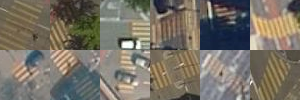
\includegraphics{images/Zebrastreifen_examples.png}
	\caption[Beispiele für Fussgängerstreifen]{6 x 2 Beispiele für Fussgängerstreifen. Wie auf den Bildern zu sehen ist, verdecken immer wieder Gegenstände das gelbe Muster. Die unterschiedliche Bildqualität der Orthofotos behinderte das Erkennen stark.}
\end{figure}

\begin{figure}[H]
	\centering
	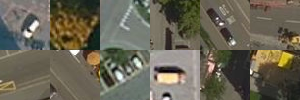
\includegraphics{images/No_Zebrastreifen_examples.png}
	\caption[Beispiele für Nicht-Fussgängerstreifen]{6 x 2 Beispiele für Nicht-Fussgängerstreifen. Das Nicht-Fussgängerstreifen Set beinhaltet alle möglichen Strassensituationen von Stadt bis Land. Besonders bei gelben Autos oder Strassenmarkierungen hat das Convnet mühe.}
\end{figure}

Ein Beispiel für ein Training eines Convnets kann unter der Datei examples/ConvnetTrainer.py eingesehen werden. Die detaillierte Beschreibung der Funktionsweise eines Neuronalen Netzes würde den Rahmen dieser Arbeit sprengen. Eine genaue Beschreibung der Abläufe kann aus den Vorlesungsunterlagen von Stanford \cite{Convolutional} genommen werden. Das in dieser Arbeit benutzte Netz ist unter dem Namen VGGNet (Karen Simonyan, Andrew Zisserman 2014)\cite{Deep} bekannt. Es wurde Ende 2014 veröffentlicht und ist seit diesem Zeitpunkt eines der besten Neuronalen Netze für Bilderkennung. Ein mithilfe der Library Keras trainiertes Neuronales Netz kann in eine .hdf5 Datei abgespeichert werden. Nach dem Laden der Datei kann man das trainierte Netz dann immer wieder verwenden.

\subsubsection{Convnet Klasse}
Die Klasse src/detection/deep/Convnet.py wrappt das neuronale Netz in eine einfach zu verwendende Klasse ein.
\begin{python}
	   from src.detection.deep.Convnet import Convnet
	   
	1. convnet = Convnet.from_verbose(verbose=True)
	2. convnet.initialize()
	3. convnet.treshold = 0.7
	
	4. result_list = convnet.predict_crosswalks(pil_image_list)
\end{python}
\begin{enumerate}
	\item Konstruiert die Convnet Klasse mit einer Factory
	\item Lädt das gespeichert Neuronale Netz mithilfe der .hdf5 Datei. Keras übersetzt das Netz in diesem Schritt in C++ und kompiliert es. Die Ausführung ist dementsprechend schnell.
	\item Manuelles setzen eines Schwellwerts. Der Schwellwert muss zwischen 0 und 1 liegen. Standartmässig ist er auf 0.9 gesetzt. Somit muss das Netz zu 90\% sicher sein, dass es ein Fussgängerstreifen ist. Dieser Wert ergab in unseren Experimenten die besten Resultate.
	\item Kategorisiert eine Liste von 50 x 50 Pixel RGB PIL Bilder. Diese Funktion nimmt eine Liste entgegen, da Keras die Bilder so parallel auf mehreren CPU Kernen verarbeiten kann. Als Rückgabewert erhält result\_list eine Liste von Booleans.
\end{enumerate}

\subsubsection{Zebrasteifenerkennung entlang der Strassen}
In diesem Abschnitt kommen die Strasseninformationen, Orthofotos, Inputbilder und das Convnet zusammen. Die Klassen StreetWalker und BoxWalker stellen Funktionen zur Verfügung, mithilfe derer alle Strassen innerhalb einer Bounding Box entlang "'gelaufen"' und die Fussgängerstreifen erkannt werden.

\subsubsection{StreetWalker}
Der StreetWalker löst das Erkennungsproblem entlang eines Strassenabschnitts. Ein Strassenabschnitt besteht aus zwei Koordinaten. Der Walker geht von der ersten Koordinate auf die zweite Koordinate zu entlang einer geraden Linie. Zum Schluss fasst er doppelt gefundene Fussgängerstreifen mithilfe des NodeMergers zusammen (siehe unten).
\begin{python}
	from src.detection.StreetWalker import StreetWalker
	
	1. walker = StreetWalker.from_street_tile(street, tile, convnet)
	2. crosswalks = walker.walk()
\end{python}
\begin{enumerate}
	\item Erstelle einen StreetWalker anhand eines Strassenabschnitts, des Orthofotos und des Convnets.
	\item Walker läuft entlang dieses Strassenabschnitts und gibt eine Liste von Koordinaten der gefundenen Fussgängerstreifen zurück.
\end{enumerate}

\subsubsection{BoxWalker}
Der BoxWalker löst das Erkennungsproblem für eine ganze Bounding Box. Zuerst lädt er die Orthofotos, die Strassen- und Fussgängerstreifeninformationen herunter. Danach erfolgt der eigentliche Erkennungsprozess, indem er für jeden Strassenabschnitt einen Streetwalker initialisiert. Zu guter Letzt vergleicht er die gefundenen Fussgängerstreifen mit den bestehenden aus OpenStreetMap und lässt den NodeMerger doppelt gefundene Fussgängerstreifen zusammenfassen (siehe unten).

\begin{python}
	from src.detection.BoxWalker import BoxWalker
	
	1. rapperswil = Bbox.from_bltr(47.224553, 8.816052, 47.227839, 8.820165)
	
	2. walker = BoxWalker(rapperswil)
	3. walker.load_convnet()
	4. walker.load_tiles()
	5. walker.load_streets()
	
	6. walker.walk()
	
	7. all_crosswalk_nodes = walker.plain_result
	8. compared_crosswalk_nodes = walker.compared_with_osm_result
\end{python}
\begin{enumerate}
	\item Erstelle eine Bounding Box anhand von Koordinaten.
	\item Erstelle einen BoxWalker mit der BBox.
	\item Lade das Convnet.
	\item Lade die Orthofotos.
	\item Lade die Strasseninformationen.
	\item Eigentlicher Erkennungsprozess.
	\item In plain\_result sind nun alle gefundenen Fussgängerstreifen enthalten.
	\item In compared\_with\_osm\_result sind nur noch die Fussgängerstreifen enthalten, die nicht schon in OpenStreetMap vorhanden sind.
\end{enumerate}

\subsubsection{NodeMerger}
Die NodeMerger-Klasse versucht das Problem der doppelten Erkennung zu lösen. Dadurch, das sich die Inputbilder überlappen, kann es dazu kommen, das Fussgängerstreifen doppelt erkannt werden. Das gleiche Problem tritt auf, wenn mehrere Strassen über den gleichen Fussgängerstreifen führen.
\\
\begin{figure}[H]
	\centering
	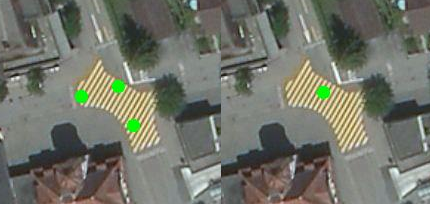
\includegraphics{images/NodeMerger_Beispiel.png}
	\caption[Beispiele NodeMerger]{Beispiel NodeMerger - Dieser Fussgängerstreifen liegt auf einer Kreuzung und ist ziemlich gross. Links vor der Zusammenfassung, rechts danach. Der Merger nimmt den Durchschnitt aller drei Koordinaten als neue Koordinate.}
\end{figure}


Der NodeMerger nimmt alle gefundenen Koordinaten entgegen und berechnet alle Abstände von gefundenem Fussgängerstreifen zu gefundenem Fussgängerstreifen. Sind die Koordinaten genug nah beieinander, werden sie zusammengefasst. Genau genommen wird hier ein Graph mit Knoten und Kanten aufgebaut. Die Koordinaten sind die Knoten und die Knoten werden verbunden, wenn sie genug nahe beieinander sind. Zum Schluss werden alle Knoten zusammengefasst, welche verbunden sind.

Kritisch ist hier die richtige Distanz zu finden. Zu grosse Distanzen fassen mehrere Fussgängerstreifen zu einem zusammen. Zu kleine Distanzen lassen zu viele Punkte übrig.

\decision{NodeMerger Distanzen} StreetWalker: 10 Meter, BoxWalker: 7 Meter

\subsubsection{Vergleich gefundene Fussgängerstreifen mit bestehenden Fussgängerstreifen in OSM}
Der Boxwalker führt nach dem Erkennungsvorgang ein Vergleich mit den bestehenden Fussgängerstreifen in OpenStreetMap durch. Dabei rechnen wir die Distanz von den gefundenen Fussgängerstreifen zu den bestehenden Fussgängerstreifen aus. Ist die Distanz kleiner 5 Meter, so besteht der Fussgängerstreifen schon und wird in walker.compared\_with\_osm\_result nicht aufgelistet.








